% vim:encoding=utf8 ft=tex sts=2 sw=2 et:

\documentclass{classrep}
\usepackage[utf8]{inputenc}

\usepackage[pdftex]{color,graphicx}
\DeclareGraphicsExtensions{.pdf,.png,.jpg}

\usepackage{float}

\usepackage{color}

\usepackage{listings}

\usepackage{color}

\usepackage[hyphens]{url}

\usepackage{hyperref}

\usepackage[polish]{babel}

\usepackage{enumitem}


\usepackage{indentfirst}
\usepackage[center,small,bf]{caption}
\hypersetup{colorlinks=false,pdfborder={0 0 0}}

\renewcommand{\labelitemi}{$\bullet$}
\renewcommand{\labelitemii}{$\cdot$}
\renewcommand{\labelitemiii}{$\diamond$}
\renewcommand{\labelitemiv}{$\ast$}
\definecolor{dkgreen}{rgb}{0,0.6,0}
\definecolor{gray}{rgb}{0.5,0.5,0.5}
\definecolor{mauve}{rgb}{0.58,0,0.82}
\lstset{ %
  language=Matlab,                % the language of the code
  basicstyle=\footnotesize,           % the size of the fonts that are used for the code
  numbers=left,                   % where to put the line-numbers
  numberstyle=\tiny\color{gray},  % the style that is used for the line-numbers
  stepnumber=2,                   % the step between two line-numbers. If it's 1, each line 
                                  % will be numbered
  numbersep=5pt,                  % how far the line-numbers are from the code
  backgroundcolor=\color{white},      % choose the background color. You must add \usepackage{color}
  showspaces=false,               % show spaces adding particular underscores
  showstringspaces=false,         % underline spaces within strings
  showtabs=false,                 % show tabs within strings adding particular underscores
  frame=single,                   % adds a~frame around the code
  rulecolor=\color{black},        % if not set, the frame-color may be changed on line-breaks within not-black text (e.g. commens (green here))
  tabsize=2,                      % sets default tabsize to 2 spaces
  captionpos=b,                   % sets the caption-position to bottom
  breaklines=true,                % sets automatic line breaking
  breakatwhitespace=false,        % sets if automatic breaks should only happen at whitespace
  title=\lstname,                   % show the filename of files included with \lstinputlisting;
                                  % also try caption instead of title
  keywordstyle=\color{blue},          % keyword style
  commentstyle=\color{dkgreen},       % comment style
  stringstyle=\color{mauve},         % string literal style
  escapeinside={\%*}{*)},            % if you want to add a~comment within your co
}
\hyphenation{Fibonacciego}

\studycycle{Informatyka, studia dzienne, mgr II st.}
\coursesemester{I}

\coursename{Metody obliczeniowe optymalizacji}
\courseyear{2011/2012}

\courseteacher{mgr inż. Łukasz Chomątek}
\coursegroup{czwartek, 16:00}

\author{
  \studentinfo{Paweł Musiał}{178726} \and
  \studentinfo{Łukasz Michalski}{178724}
}

\title{Zadanie 2: Optymalizacja kierunkowa}
\svnurl{https://serce.ics.p.lodz.pl/svn/labs/moo/lc_cz1600/lmpm}

\begin{document}
\maketitle

\addtocounter{footnote}{1}

\section{Cel}
Celem zadania było napisać program, który dla dowolnej funkcji dwóch zmiennych rozwiąże zadanie optymalizacji na odcinku. Optymalizacja kierunkowa musi być przeprowadzona z wykorzystaniem kryteriów:
\begin{itemize}
\item Armijo
\item Wolfa
\item Goldsteina
\end{itemize}
Przedstawiany jako rozwiązanie program powinien pozwolić wprowadzić funkcję oraz odcinek, w którym poszukiwane będzie rozwiązanie.

\section{Rozwiązanie zadania}
\subsection{Metoda najszybszego spadku}
Metoda najszybszego spadku jest iteracyjnym algorytmem wyszukiwania minimum zadanej funkcji celu $f$. Założenia dla metody są następujące:
\begin{itemize}
\item $f\in C^1$ (funkcja jest ciągła i różniczkowalna),
\item $f$ jest ściśle wypukła w badanej dziedzinie.
\end{itemize}
Poszukiwania te odbywają się na podstawie gradientu tej funkcji. Wiadomo, że gradient $\bigtriangledown f=[\frac{\partial f}{\partial x_{1}},...,\frac{\partial f}{\partial x_{n}}]^T$ ma ważną własność mówiącą że poruszając się z dowolnego punktu $x$ ,,w kierunku gradientu'' osiągamy (lokalnie) najszybszy przyrost funkcji. W myśl tej zasady, jeśli $\bigtriangledown f$ wyznacza najszybszy wzrost, to $-\bigtriangledown f$ wyznacza najszybszy spadek. Na tym spostrzeżeniu opiera się metoda najszybszego spadku, którą w skrócie można ja opisać następująco:
\begin{enumerate}
\item Znajdź najlepszy kierunek (kierunek najszybszego spadku),
\item Określ jak daleko chcesz ,,zrobić krok'' w tym kierunku,
\item Zrób krok i sprawdź warunek stopu.
\end{enumerate}

Problemem występującym przy zastosowaniu metody najszybszego spadku jest jej ,,spowolnienie'', gdy zbliża się do minimum (zmiany zmiennych zależna od wielkości gradientu, a gradient dąży do zera w otoczeniu punktu minimum). Alogrytm działania tej metody został przedstawiony na diagramie:
\begin{figure}[h!]
\centering
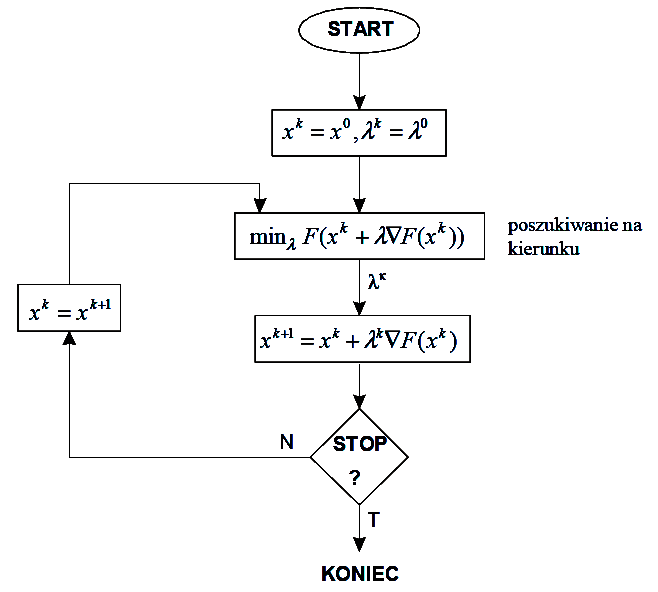
\includegraphics[width=10cm]{obrazy/metodaNS_algo} 
\caption{Schemat działania metody najszybszego spadku.\\*{\footnotesize Źródło: Wykład 4 Wojciecha Grega: Metody Optymalizacji}}
\label{fig:metodaNS_algo}
\end{figure}

Jak można zauważyć ważnym elementem tego algorytmu jest wybór odpowiedniej długość użytego kroku oraz kryterium stopu. Ma to bowiem wpływ na szybkość i stabilność działania oraz na osiągnięte wyniki. W tym zadaniu skupimy się na trzech kryteriach doboru optymalnego kroku:
\begin{itemize}
\item Armijo
\item Wolfa
\item Goldsteina
\end{itemize}

Na rysunku \ref{fig:metodaNS_przebieg} można zobaczyć przykład działania metody najszybszego spadku dla dwuwymiarowej funkcji celu. W każdym kroku, w zadanym kierunku wyszukiwana jest najmniejsza wartość funkcji celu.
\begin{figure}[h!]
\centering
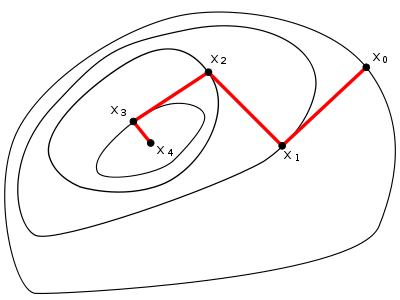
\includegraphics[width=6cm]{obrazy/metodaNS_przebieg} 
\caption{Przebieg działania metody najszybszego spadku. \\*{\footnotesize Źródło: \url{http://pl.wikipedia.org/wiki/Plik:Metoda_najszybszego_spadku.svg}}}
\label{fig:metodaNS_przebieg}
\end{figure}
\\
W opisach kryteriów zbieżności posługiwać będziemy się poniższymi oznaczeniami :
\begin{itemize}
 \item $x^k$ - kolejne przybliżenia rozwiązania
 \item $\lambda ^k$ - długość kroku
 \item $d ^k$ - kierunek zmiany
 \item $c$ - stałe używane w kryteriach
 \item $f(x)$ - wartość funkcji podstawowej w punkcie
 \item $\nabla f(x)$ - wartość gradientu w punkcie
\end{itemize}
\subsection{Kryterium Armijo}

\begin{equation}
f( x^{k} + \lambda ^{k} d^{k} ) \leq f(x^{k}) + c \lambda ^{k} \nabla f^{T} (x ^{k} ) d^{k}
\end{equation}

Warunek ten oznacza, że redukcja wartości funkcji celu powinna być proporcjonalna do długości kroku jak również do pochodnej kierunkowej. Metoda ta jednak nie zapewnia nam szybkiej zbieżności, ponieważ zawsze może być spełniony dla dostatecznie małej wielkości $\lambda$ 

\subsection{Kryterium Wolfa}

Kryterium Wolfa, jest rozszerzeniem kryterium poprawy Armijo, o kryterium krzywizny :
\begin{itemize}
\item Słabe kryterium krzywizny\\
	\begin{equation}
	\nabla f^{T} (x^{k} + \lambda ^{k} d^{k} ) d^{k} \geq c \nabla f^{T} (x ^{k} ) d^{k}
	\end{equation}
	
\item Silne kryterium krzywizny\\
	\begin{equation}
	\| \nabla f^{T} (x^{k} + \lambda ^{k} d^{k} ) d^{k} \| \leq \| c \nabla f^{T} (x ^{k} ) d^{k} \|
	\end{equation}

\end{itemize}

Kryterium to zapewnia nam, że gdy w punkcie początkowym jest duży spadek, nie będzie wykonany mały krok.


\subsubsection{Słabe kryterium Wolfa}

\begin{equation}
	\nabla f^{T} (x^{k} + \lambda ^{k} d^{k} ) d^{k} \geq c \nabla f^{T} (x ^{k} ) d^{k}  \ \ \&\& \ \ 
	f( x^{k} + \lambda ^{k} d^{k} ) \leq f(x^{k}) + c \lambda ^{k} \nabla f^{T} (x ^{k} ) d^{k}
\end{equation}

Jest to kryterium Armijo z dodatkowym założeniem słabego kryterium krzywizny.

\subsubsection{Silne kryterium Wolfa}

\begin{equation}
	\| \nabla f^{T} (x^{k} + \lambda ^{k} d^{k} ) d^{k} \| \leq \| c \nabla f^{T} (x ^{k} ) d^{k} \| \ \ \&\& \ \ 
	f( x^{k} + \lambda ^{k} d^{k} ) \leq f(x^{k}) + c \lambda ^{k} \nabla f^{T} (x ^{k} ) d^{k}
\end{equation}

Jest to kryterium Armijo z dodatkowym założeniem silnego kryterium krzywizny.

\subsection{Kryterium Goldsteina}

\begin{equation}
f( x^{k} ) + (1-c) \lambda ^{k} \nabla f(x^{k}) d^{k} \leq f(x^{k}+ \lambda ^{k} d^{k} ) \leq f(x^{k}) + c \lambda ^{k} \nabla f(x^{k} ) d^{k}
\end{equation}

Kryterium Goldsteina, podobnie jak w przypadku kryterium Wolfa, zabezpiecza nas przed zbyt małym krokiem, który mógłby niepotrzebnie zwiększyć ilość potrzebnych iteracji. Lewa i prawa część nierówności zapewnia nam ograniczenie odpowiednio dolnej i górnej granicy kroku.

\subsection{Algorytm backtrackingu}
Jest metodą wyznaczania długości kroku na podstawie zadanego kryterium.
\begin{enumerate}
\item sprawdź czy zachodzi kryterium dla zadanej długości kroku
\item jeśli kryterium zachodzi, zwróć długość kroku $\lambda$
\item jeśli kryterium nie zachodzi, oblicz $\lambda=\lambda \ro$, gdzie $\ro \in (0,1)$ , wróć do 1
\end{enumerate}



\section{Opis programu}
Program w całości jest implementacja powyżej opisanych metod. 
Wyjaśnienie znaczenia zmiennych :
\begin{itemize}
\item f0 - funkcja podstawowa
\item f1 - gradient funkcji
\item p - kierunek zmiany
\item x - kolejne przybliżenia
\item a - długość kroku
\item c - parametr kryterium
\item rho - parametr backtrackingu
\end{itemize}

\subsection{Metoda najszybszego spadku}

\begin{lstlisting}{Metoda najszybszego spadku}
function x=steepest_descent(x0,sl,fn,a0,rho,c)
f=inline(fn);
f0=@(x)f(x(1),x(2));
t=[x;y];
w=fn;
gfn=matlabFunction(jacobian(w,t).');
f1=@(x)gfn(x(1),x(2));
while k<10 %warunek zakończenia, liczba iteracji
    %kierunek
    p=-f1(x);
    %długość kroku spełniająca kryterium
    a=kryterium(x,p);
    %kolejne przybliżenie
    x=x+a*p
    %licznik iteracji
    k=k+1;
end
\end{lstlisting}

\subsection{Kryterium Armijo}

\begin{lstlisting}{Kryterium Armijo}
if f0(x+a*p)<=f0(x)+c*a*f1(x)'*p
    test=1;
else 
    test=0;
end
\end{lstlisting}


\subsection{Kryterium Wolfa}

\begin{lstlisting}{Słabe kryterium Wolfa}
if c(1)*f1(x)'*p<=f1(x+a*p)'*p &&
 f0(x+a*p)<=f0(x)+c(2)*a*f1(x)'*p
    test=1;
else 
    test=0;
end
\end{lstlisting}

\begin{lstlisting}{Silne kryterium Wolfa}
if abs(c(1)*f1(x)'*p)>=abs(f1(x+a*p)'*p) &&
 f0(x+a*p)<=f0(x)+c(2)*a*f1(x)'*p
    test=1;
else 
    test=0;
end
\end{lstlisting}


\subsection{Kryterium Goldsteina}

\begin{lstlisting}{Kryterium Goldsteina}
if f0(x+a*p)<=f0(x)+c*a*f1(x)'*p &&
 f0(x+a*p)>=f0(x)+(1.0-c)*a*f1(x)'*p
    test=1;
else 
    test=0;
end
\end{lstlisting}


\subsection{Algorytm backtrackingu}

\begin{lstlisting}{Algorytm backtrackingu}
switch cond
    case 'armijo'
        check=@(a)armijo(a,x,p,c,f0,f1);
    case 'goldstein'
        check=@(a)goldstein(a,x,p,c,f0,f1);
    case 'wolfe'
        check=@(a) wolfe(a,x,p,c(1),f1) &&
        			 armijo(a,x,p,c(2),f0,f1);
    case 'wolfes'
        check=@(a) wolfes(a,x,p,c(1),f1) &&
        			 armijo(a,x,p,c(2),f0,f1);
end
a=a0;
while check(a)~=1  %poszukiwanie długości kroku dla której
                   %zachodzić będzie dane kryterium
    a=rho*a;
end

\end{lstlisting}

\section{Wyniki}
	
\section{Wnioski}

\begin{thebibliography}{9}
\bibitem{1}
	Michał Lewandowski,  \emph{Metody optymalizacji - teoria i~wybrane algorytmy}.  2012.
\end{thebibliography}

\end{document}